\documentclass[../main.tex]{subfiles}
\graphicspath{{\subfix{../IMAGES/}}}

\begin{document}
\localtableofcontents

\subsection{Circuit magnétique}
\subsubsection{Équations de Maxwell (quasi-statique)}
\begin{itemize}
    \item S'il y a un courant, il y a un champ magnétique : (loi d'Ampère) $\oint_C \mathbf{H}\cdot \mathbf{dl} = \int_S \mathbf{J}\cdot \mathbf{dS} = \sum_j i_j$\\
    \item S'il y a une variation du flux, il y a une tension induite : (loi de Lenz-Faraday) $\oint_C \mathbf{E}\cdot \mathbf{dl} = -\int_S \frac{\partial \mathbf{B}}{\partial t}\cdot \mathbf{dS}$\\
    \item Pas de monopole magnétique mais des paires de pôles : $\oint_S \mathbf{B}\cdot \mathbf{dS}=0$\\
\end{itemize}

\quad \underline{Modèle de Kirchhoff :} il y a équivalence entre le monde électrique et magnétique \begin{itemize}
    \item Potentiel magnétique $\rightarrow$ tension\\
    \item Flux d'induction magnétique $\rightarrow$ courant\\
    \item Perméance $\rightarrow$ inverse de la résistance\\
\end{itemize}

\subsubsection{Potentiel magnétique scalaire}
\begin{equation}
    \theta = \oint_C \mathbf{H \cdot dl} = Hl = Ni [A]
\end{equation}
Avec N, le nombre de boucles.

\subsubsection{Champ d'induction magnétique}
\begin{equation}
    \mathbf{B} = \mu \mathbf{H}
\end{equation}
Avec B le champ d'induction magnétique, H le champ magnétique (indépendant du milieu) et $\mu$ la perméabilité du matériau.\\

\begin{equation}
    \mu = \mu_r \mu_0
\end{equation}
$\mu_r$ la perméabilité relative et $\mu_0 = 4\pi 10^{-7}$ la perméabilité du vide.\\

\warning Pour les matériaux ferromagnétiques on trouve un coude de saturation au dessus duquel la relation entre B et H n'est plus linéaire.\\

\subsubsection{Flux d'induction magnétique}
\begin{equation}
\begin{split}
    \phi = \int_S \mathbf{B\cdot dS} = BS [Vs]\\
    \psi = N \phi \text{le flux totalisé}
    \end{split}
\end{equation}

\subsubsection{Réluctance et perméance magnétique}
\underline{Réluctance magnétique :}\begin{equation}
    R_m = \int_A^B \frac{dl}{\mu_0\mu_r S} = \frac{l}{\mu S}
\end{equation}

\underline{Perméance magnétique :}\begin{equation}
    \Lambda = \frac{1}{R_m} = \mu \frac{S}{l} [H]
\end{equation}

Enfin, on a \begin{equation}
    \phi = \Lambda \theta
\end{equation}

\begin{itemize}
    \item Mise en parallèle de perméances : $\Lambda_{eq} = \sum_k \Lambda_k$\\
    \item Mise en série de perméances : $\Lambda_{eq} = \frac{1}{\sum_k \frac{1}{\Lambda_k}}$\\
\end{itemize}

\subsubsection{Inductances}
\begin{equation}
    \psi = Li
\end{equation}
Une inductance agissant sur une autre peut se diviser en en une inductance de champ principal et une inductance de fuite.\\
\begin{equation}
    \text{inductance propre } L_{11} = L_{hl}+L_{\sigma l} [H]
\end{equation}
Avec \begin{itemize}
    \item $L_{hl} = N_1^2 \Lambda_{hl}$ l'inductance de champ principal\\
    \item $L_{\sigma l} = N_1^2 \Lambda_{\sigma l}$ l'inductance de fuite\\
\end{itemize}

On a également une inductance mutuelle : \begin{equation}
    L_{12} = L_{21} = N_1 N_2 \Lambda_{12}
\end{equation}


\subsubsection{Tension induite}
Loi d'Ohm généralisée : \begin{equation}
    u = Ri+ \frac{d\psi}{dt}
\end{equation}

\begin{itemize}
    \item Tension dans une bobine lorsqu'un courant la traverse avec une autre bobine à côté : $u_1 = R_1 i_1 + L_{11} \frac{di_1}{dt} + L_{12} \frac{di_2}{dt}$\\
    \item Tension dans une bobine lorsqu'un aimant translate ou est en rotation à côté (ex : rotor dans stator) $u_1 = Ri + L \frac{di}{dt} + k_{\phi} \Omega$\begin{itemize}
        \item $L \frac{di}{dt}$ : la tension induite de transformation\\
        \item $k_\phi \Omega$ : la tension induite de mouvement ($\Omega$ la vitesse de rotation)\\
    \end{itemize} 
\end{itemize}

\subsection{Transformateur}
Le transformateur : transforme un système de tension/courant variable en un autre système de tension/courant de \textbf{même fréquence}.\\

\begin{figure}[hbt!]
    \centering
    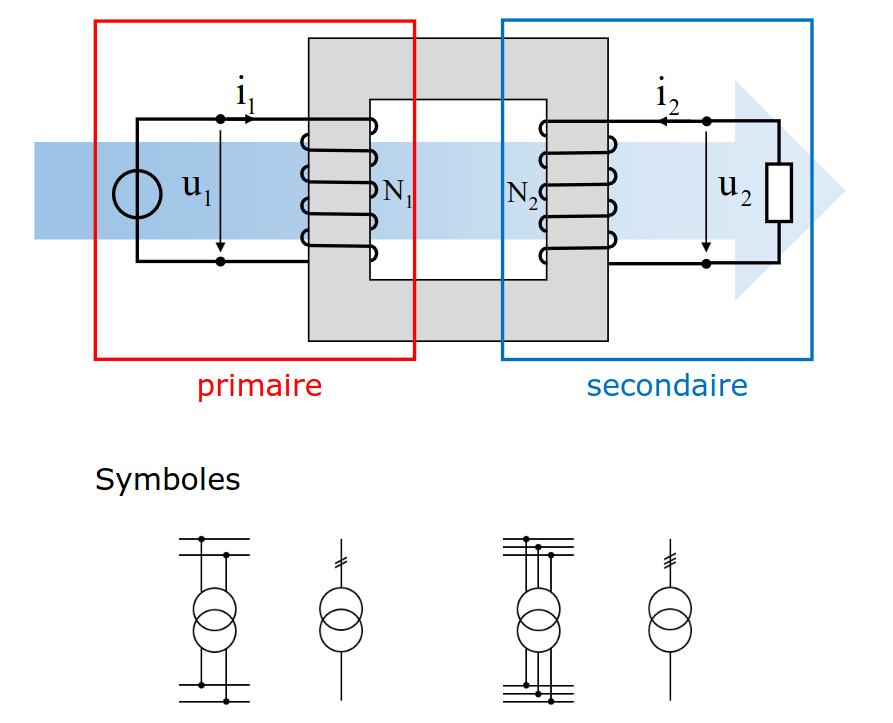
\includegraphics[width = \textwidth]{IMAGES/machineelec/transfo.png}
\end{figure}

\subsubsection{Monophasé idéal}
Hypothèses : \begin{itemize}
    \item Alimentation sinusoïdale\\
    \item La perméabilité du circuit magnétique est infinie : pas de flux de fuites\\
    \item La résistance des enroulements est négligée\\
\end{itemize}

\begin{equation}
    \begin{cases}
        u_1 = \frac{d\psi_1}{dt} = N_1 \frac{d\phi}{dt}\\
        u_2 = \frac{d\psi_2}{dt} = N_2 \frac{d\phi}{dt}\\
    \end{cases}
\end{equation}

Rapport de transformation : \\
\begin{equation}
    \frac{N_1}{N_2} = \frac{U_1}{U_2} = -\frac{I_2}{I_1} = \Ddot{u}
\end{equation}

Soit $\underline{Z}_{ch}$ l'impédance d'une charge sur le circuit secondaire, on cherche son effet sur le circuit primaire, à savoir $\underline{Z}_{ch}'$ : \begin{equation}\begin{split}
    \underline{Z}_{ch}' = (\frac{N_1}{N_2})^2 \underline{Z}_{ch} = \Ddot{u}^2 \underline{Z}_{ch}\\
    \underline{U}_2' = \Ddot{u}\underline{U}_2\\
    \underline{I}_2' = \frac{1}{\Ddot{u}}\underline{I}_2
    \underline{S}_1 = -\underline{S}_2 \text{La puissance apparente}
    \end{split}
\end{equation}

\subsubsection{Monophasé réel}
Équations de tensions : \begin{equation}
    \begin{split}
        \begin{cases}
            u_1 = R_1 i_1 + L_{hl} \frac{di_1}{dt} + L_{\sigma l} \frac{di_1}{dt} + L_{12} \frac{di_2}{dt}\\
            u_2 = R_2 i_2 + L_{hl} \frac{di_2}{dt} + L_{\sigma l} \frac{di_2}{dt} + L_{12} \frac{di_1}{dt}\\
        \end{cases}\\
        \begin{cases}
            \underline{U}_1 = R_1 \underline{I}_1 + j \omega L_{hl} \underline{I}_1 + j \omega L_{\sigma l} \underline{I}_1 + j\omega L_{hl} \underline{I}_2'\\
            \underline{U}_2' = R_2' \underline{I}_2' + j \omega L_{hl} \underline{I}_2' + j \omega L_{\sigma l}' \underline{I}_2' + j\omega L_{hl} \underline{I}_1\\
        \end{cases}\\
        \begin{cases}
            \underline{U}_1 = R_1 \underline{I}_1 + j X_h \underline{I}_1 + j X_{\sigma 1} \underline{I}_1 + j X_{h} \underline{I}_2'\\
            \underline{U}_2' = R_2' \underline{I}_2' + j X_{h} \underline{I}_2' + j X_{\sigma 2} \underline{I}_2' + j X_{h} \underline{I}_1\\
        \end{cases}
    \end{split}
\end{equation}

On dénote ici d'un prime les valeurs rapportés au primaire (la charge qu'émet un élément sur le réseau fournissant l'énergie).\\

\quad \underline{Pertes fer :} $P_{\text{fer}} = P_{\text{hystérèsis}} + P_{\text{courants de Foucault}}$\\

\quad \underline{Fonctionnement en court-circuit :} On peut rassembler le circuit en un seul : 

\begin{figure}[hbt!]
    \centering
    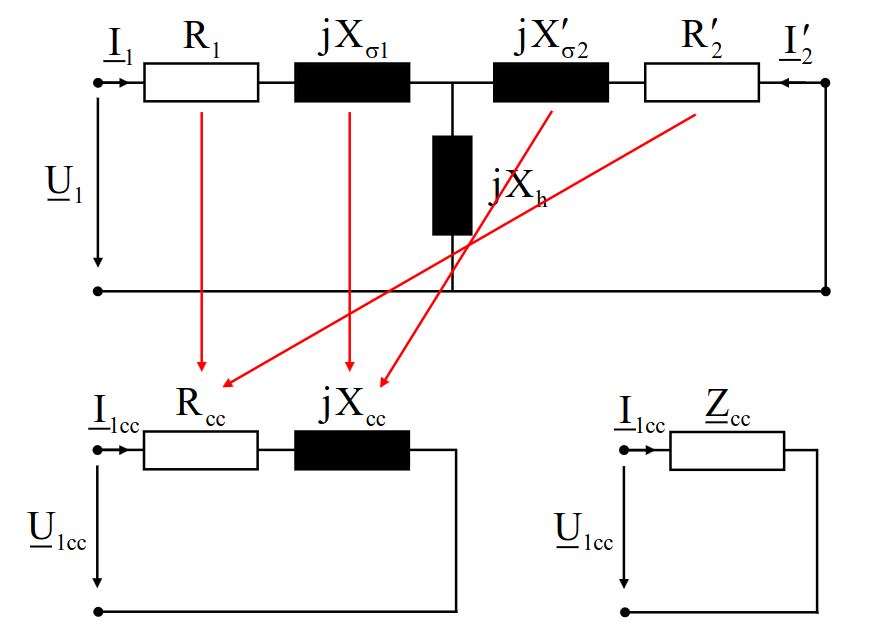
\includegraphics[width=\textwidth]{IMAGES/machineelec/courtcircuit.png}
\end{figure}

Ainsi : \begin{itemize}
    \item $R_{cc} = R_1 + R_2'$\\
    \item $X_{cc} = X_{\sigma 1} + X_{\sigma 2}'$\\
    \item $\underline{Z}_{cc} = R_{cc} + jX_{cc}$\\
\end{itemize}

\quad \underline{Hypothèse de Kapp :}\\

\begin{figure}[hbt!]
    \centering
    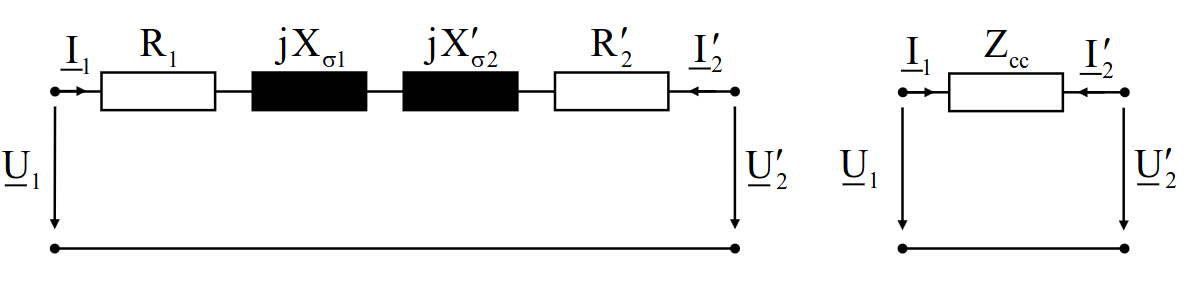
\includegraphics[width=\textwidth]{IMAGES/machineelec/kapp.png}
\end{figure}

\begin{itemize}
    \item $\underline{I}_1 = -\underline{I}_2'$\\
    \item $\underline{U}_1 = \underline{Z}_{cc} \underline{I}_1 + \underline{U}_2'$\\
    \item $u_{cc} = \frac{U_{lcc}}{U_{ln}}$ [pu]\\
    \item $Z_{cc} = \frac{U_{lcc}}{I_{lcc}} = \frac{U_{lcc}}{I_{ln}}$\\
    \item $z_{cc} = u_{cc}$\\
    \item $R_2' = \Ddot{u}^2 R_2$ (de même pour $X_{\sigma2}'$)\\
    \item $I_{ch} = \Ddot{u} I_{ch}'$\\
\end{itemize}


\subsubsection{Puissances triphasées}
\begin{itemize}
    \item Puissance apparente $S = 3U_{ph} I_{ph} = \sqrt{3}U_{ligne} I_{ligne} = \sqrt{P^2+Q^2}[VA]$\\
    \item Puissance active $P = S \cos{\phi} [W]$\\
    \item Puissance réactive $Q = S \sin{\phi} [VAr]$\\ 
\end{itemize}

\begin{itemize}
    \item Moteur inductif : $P>0$, $Q>0$\\
    \item Moteur capacitif : $P>0$, $Q<0$\\
    \item Génératrice capacitive : $P<0$, $Q<0$\\
    \item Génératrice inductive : $P<0$, $Q>0$\\
\end{itemize}

\begin{table}[hbt!]
    \centering
    \begin{tabular}{|c|c|c|}
    \hline
    \multicolumn{1}{|c|}{\diagbox[width=7mm,height=5mm]{\diagbox[width=7mm,height=5mm,dir=SW]{}{}}{}} & Étoile & Triangle \\
    \hline
    $U_l$ & $\sqrt{3}U_{ph} $ & $U_{ph}$\\
    \hline
    $I_l$ & $I_{ph}$ & $\sqrt{3} I_{ph}$\\
    \hline
    $I_{ph}$ & $\frac{U_{ph}}{Z} = \frac{U_l}{\sqrt{3}Z}$ & $\frac{U_{l}}{Z}$ \\
    \hline
    P & $3 U_{ph} I_{ph} cos(\varphi)$ & $3 U_{ph} I_{ph}cos(\varphi)$\\
    \hline

    \end{tabular}
    \caption{Conversion Étoile/Triangle}
    
\end{table}

\subsection{Éléments de base des machines}
Génération d'un couple par interaction de champs magnétiques.\\
Une machine électrique est constitué d'un stator (partie fixe) et d'un rotor (partie tournante).\\
Un rotor peut être formé d'une bobine (électro-aimant) ou d'un aimant permanent.\\
Le champ d'induction magnétique au stator est créé par un courant électrique présent dans un enroulement (bobines).\\

Le stator est constitué de fer feuilleté.\\

\quad \underline{Génération d'un couple par interaction de champs magnétiques :}\\
Il s'agit ici d'un \textbf{couple électromagnétique}.\\

\begin{equation}
    T_{em} = k B_s B_r p \sin{\delta}
\end{equation}
Avec \begin{itemize}
    \item k : un facteur géométrique\\
    \item $B_s$ : le champ du stator\\
    \item $B_r$ : le champ du rotor\\
    \item $p$ : le nombre de paires de pôles\\
\end{itemize}

Deux conditions:\begin{itemize}
    \item Même nombre de pôles (paires de pôles)\\
    \item Même vitesse (les champs sont synchrones)\\
\end{itemize}

\quad \underline{Action d'un champ magnétique sur une structure à réluctance variable :}\\
Il s'agit ici d'un \textbf{couple réluctant}.\\

\begin{equation}
    T_{em} = k B_s^2p \sin(2\delta)
\end{equation}
Deux conditions : \begin{itemize}
    \item Même nombre de pièces saillantes que de pôles\\
    \item Même vitesse\\
\end{itemize}

Il faut ici une structure de rotor spéciale pour avoir une rotation. Les champs du stator vont d'un Nord vers un Sud mais préfèrent passer à travers le fer du rotor qui va s'orienter dans selon les lignes de champs et donc induire un torque.\\

Dans la plupart des moteurs, on utilise une combinaison des deux phénomènes.\\

\subsubsection{Champ tournant}
On fait passer dans une bobine un courant : $i(t) = \sqrt{2}I \cos{\omega t}$.\\
\begin{figure}[hbt!]
    \centering
    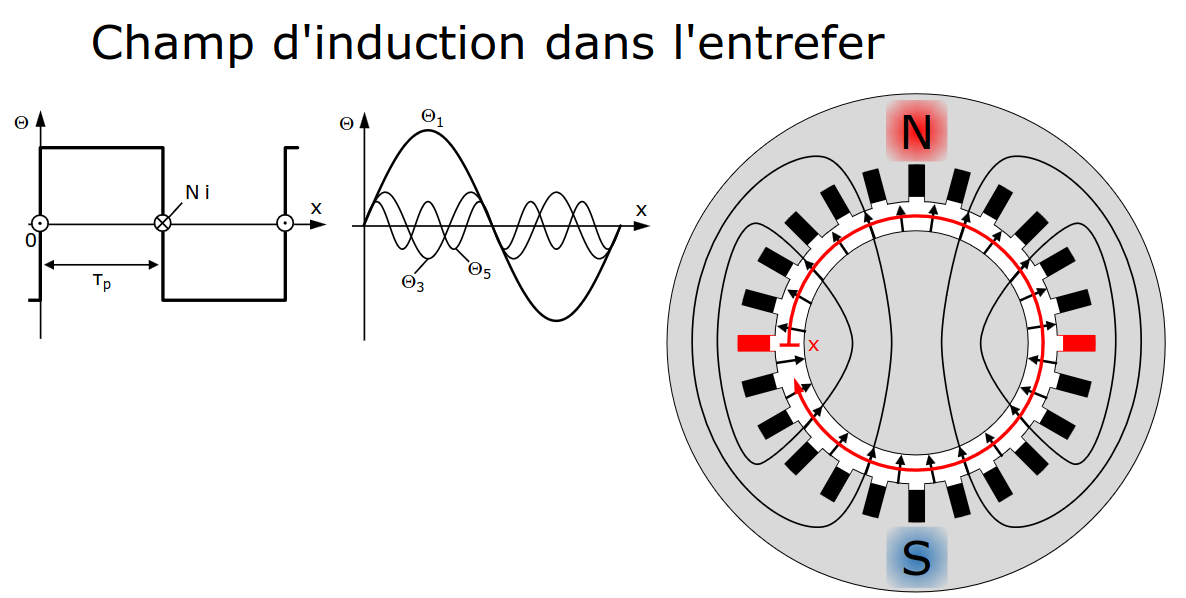
\includegraphics[width=\textwidth]{IMAGES/machineelec/bobenf.png}
\end{figure}

Le champ d'induction généré dans l'entrefer équivaut à un signal carré selon l'axe curviligne $x$. Celui-ci peut s'exprimer comme une somme de sinus. \begin{equation}
    \begin{gathered}
        \Theta_v = \frac{4 \sqrt{2}}{\pi} \frac{1}{v} NI\\
        \Theta = (\sum_v \Theta_v \sin(\frac{vx}{\tau_p}\pi))\cos{\omega t}\\
    \end{gathered}
\end{equation}

Le champ généré est donc : $B_\delta(x,t) = \mu_0 \frac{\Theta(x,t)}{2\delta}$\\

On s'intéresse uniquement à la fréquence fondamentale car elle possède la plus grande amplitude : \begin{equation}
    B_\delta (x,t) = \frac{\mu}{\delta} \frac{4}{\pi \sqrt{2}} NI \sin(\frac{x}{\tau_p}\pi) \cos(\omega t)
\end{equation}

Si l'alimentation est en triphasé (décalé de $120^\circ$ géométriquement et temporel) alors : \begin{equation}
    B_\delta(x,t) = \frac{3}{2} B \sin(\frac{\pi x}{\tau_p}\pm \omega t)
\end{equation}

Pour une alimentation biphasée (décalé de $90^\circ$ temporel et géométrique) alors : \begin{equation}
    B_\delta(x,t) = B \sin(\frac{\pi x}{\tau_p}\pm \omega t)
\end{equation}

\footnote{Un système monophasé nécessite deux fils, un biphasé quatre. Cependant, un système triphasé n'en nécessite que trois! Cela est dû au fait que les trois phases se compensent car décalé de $120^\circ$, il n'y a donc pas besoin de retour. Par exemple si la phase 1 demande 10A alors la deuxième et troisième auront -5A.}


\quad \underline{Vitesses et nombre de paires de pôles :}\\

\begin{equation}
\begin{gathered}
    \Omega_s = \frac{\omega_s}{p}\\
    n = \frac{f}{p}
    \end{gathered}
\end{equation}
Avec \begin{itemize}
    \item $\Omega$ rad/s : la vitesse angulaire dans le monde mécanique\\
    \item $\omega$ rad/s : la vitesse angulaire dans le monde électrique\\
    \item $f$ Hz : monde électrique\\
    \item $n$ tr/s : monde mécanique\\
    \item $N$ tr/min : monde mécanique\\
\end{itemize}

\subsubsection{Grandeurs relatives - Per Unit}
Il s'agit ici de s'affranchir des vraies grandeurs physiques en établissant des grandeurs relatives à des valeurs de références.\\

\warning Les valeurs de références sont souvent des grandeurs nominales; ce pour quoi est dimensionné pour un dimensionnement à vie et non pas une grandeur maximale!\\

\subsection{Machine asynchrone}
Une machine asynchrone est une machine à courant alternatif dont la vitesse en charge et la fréquence du réseau auquel elle est reliée ne sont pas dans un rapport constant.\\

Le rotor peut être soit : \begin{itemize}
    \item bobiné\\
    \item à cage d'écureuil : aluminium en forme de spire (barre rotorique) relié à des anneaux de court-circuit aux deux extrémités et comblé par du fer feuilleté\\
\end{itemize}

Si le champ tournant du stator et le rotor tournent à la même vitesse, alors $\frac{d\psi}{dt}=0$ et comme le rotor est constitué de spires court-circuitées sur elles mêmes on a : $0 = R_r i_r + \frac{d\psi}{dt}$\\

Lorsque le rotor tourne moins vite que le champ tournant du stator, le courant induit au rotor à une fréquence de $f_s-f_m$.\\

Dès lors, \textbf{les deux champs stator et rotor ont la même fréquence et leurs interaction génère le couple.} Plus le glissement est grand, plus le courant induit est grand et donc plus le champ B est grand et plus le couple est grand.\\

\subsubsection{Glissement}
Le glissement est l'écart de vitesse entre le champ tournant statorique et la vitesse mécanique du rotor rapporté à la vitesse du champ tournant statorique.\\

\begin{equation}
    s = \frac{\Omega_s-\Omega_m}{\Omega_s} = \frac{\omega_s-\omega_m}{\omega_s} = \frac{n_s-n_m}{n_s} = \frac{N_s-N_m}{N_s} = \frac{f_s-f_m}{f_s}
\end{equation}

\subsubsection{Schéma équivalent}
\begin{figure}[hbt!]
    \centering
    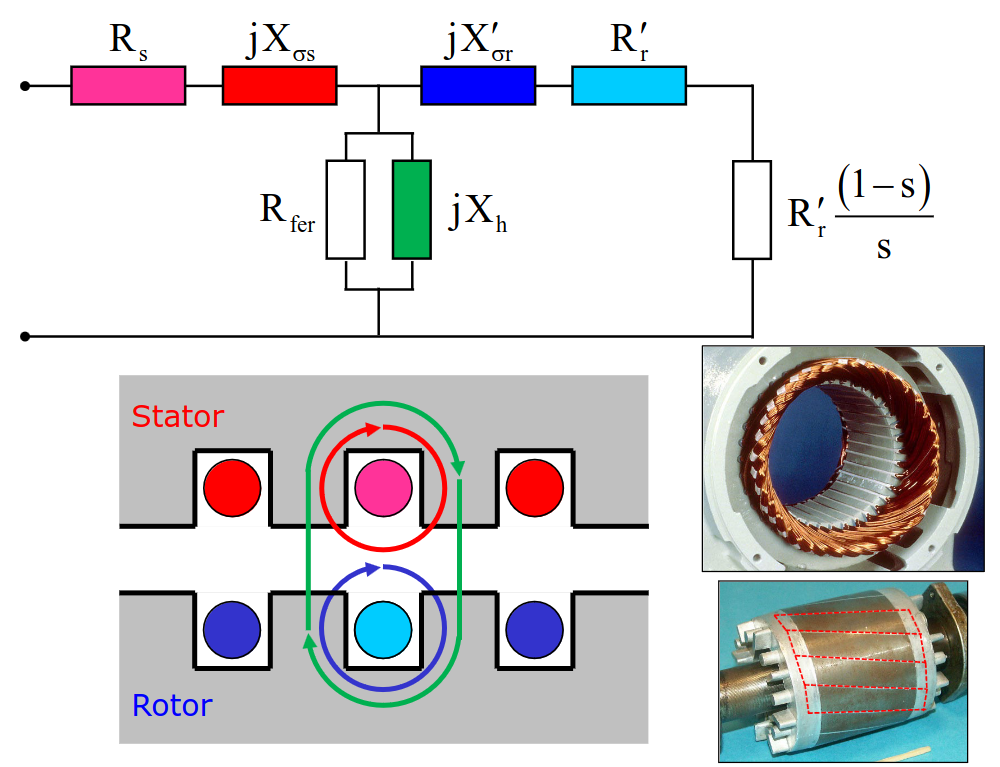
\includegraphics[width=.5\textwidth]{IMAGES/machineelec/async.png}
\end{figure}

On peut négliger les pertes fer ($R_f$).\\

On obtient les équations de tension : \begin{equation}
    \begin{gathered}
        \underline{U}_s = R_s \underline{I}_s + j X_{\sigma s} \underline{I}_s + jX_h (\underline{I}_s + \underline{I}_r' )\\
        0 = \frac{R_r'}{s} \underline{I}_r' + jX_{\sigma r}' \underline{I}_r' + jX_h(\underline{I}_s + \underline{I}_r')\\
        \omega_r = s\omega_s\\
    \end{gathered}
\end{equation}

Paramètres du schéma équivalent : \begin{itemize}
    \item $r_s \rightarrow 0.01-0.03$ p.u\\
    \item $x_{\sigma s} \rightarrow 0.08-0.12$ p.u\\
    \item $x_h \rightarrow 2.5-4$ p.u\\
    \item $x_{\sigma r}' \rightarrow 0.08-0.1$ p.u\\
    \item $r_r' \rightarrow 0.01-0.03$ p.u\\
\end{itemize}


Les paramètres se déterminent par différents essais : \begin{itemize}
    \item Mesure Ohmique pour $R_s$\\
    \item Essai en court-circuit pour $\frac{R_r'}{s} + jX_{\sigma r}'$ (rotor bloqué) : \begin{itemize}
        \item Soit $P_{cc}$ la puissance active totale, $U_{scc}$ la tension stator de phase, $I_s$ le courant stator de phase\\
        \item $Z_{cc} = Z_s + \frac{Z_h Z_r'}{Z_h+Z_r'}$ Avec : $\begin{cases}
            Z_s = R_s + jX_{\sigma s}\\
            Z_h = \frac{jR_{fer}X_h}{R_{fer} + jX_h}\\
            Z_r' = R_r' + jX_{\sigma r}'\\
        \end{cases}$\\
        \item $\lvert Z_{cc} \rvert = \frac{U_{scc}}{I_s}$, $\cos \varphi = \frac{P_{cc}}{3U_{scc}I_s}$, $\begin{cases}
            R_{cc} = \lvert Z_{cc}\rvert \cos \varphi\\
            X_{cc} = \lvert Z_{cc} \rvert \sin \varphi\\
        \end{cases}$
    \end{itemize}
    \item Essai à vide pour $\frac{1}{\frac{1}{R_{fer}} + \frac{1}{jX_h}}$ : \begin{itemize}
        \item $Z_0 = R_s+jX_{\sigma s} + \frac{jR_{fer}X_h}{R_{fer} + jX_h} \rightarrow \lvert Z_0 \rvert = \frac{U_s}{I_0}$\\
        \item $\cos \varphi = \frac{P_0-P_{fv}}{3U_sI_0}$\\
        \item $\begin{cases}
            R_0 = \lvert Z_0 \rvert \cos \varphi\\
            X_0 = \lvert Z_0 \rvert \sin \varphi\\
        \end{cases}$\\
        \item $\begin{cases}
            R_{fer} = \frac{(R_0-R_s)^2+(X_0-X_{\sigma s})^2}{R_0-R_s}\\
            X_h = \frac{(R_0-R_s)^2 + (X_0-X_{\sigma s})^2}{X_0-X_{\sigma s}}\\
        \end{cases}$\\
        \item Avec $P_{fv}$ les pertes due au frottement et à la ventilation. On a $P_0 = P_{js} + P_{fer} + P_{fv}$, $P_{js} = 3R_sI_0^2$\\
    \end{itemize}
\end{itemize}

\subsubsection{Bilan de puissance}

\begin{equation}
    P_{el} = P_{js} + P_{fer} + P_{jr} + P_{fv} + P_{utile}
\end{equation}

Avec $P_{fv}+P_{utile} = P_{mec}$ la puissance mécanique.\begin{itemize}
    \item $P_{js} \simeq 6\%$\\
    \item $P_{fer} \simeq 1.5-2\%$\\
    \item $P_{jr} \simeq 5\%$\\
    \item $P_{fv} \simeq 1.5-2\%$\\
\end{itemize}

\quad \underline{Puissance d'entrefer :}\\
\begin{equation}
    P_\delta = P_{el} - P_{js}-P_{fer} = P_{mec} + P_{jr} = 3\frac{R_r'}{s}I_r^{'2}
\end{equation}

Cependant, $P_{jr} = sP_\delta$\\

\begin{equation}
    P_{mec} = (1-s)P_\delta = P_{jr} \frac{1-s}{s} = 3R_r' \frac{1-s}{s}I_r^{'2}
\end{equation}

Cependant, $P_{mec} = \Omega_m T_{em}$\\

\begin{equation}
    T_{em} = 3 \frac{1}{\Omega_s} \frac{R_r'}{s} I_r^{'2}
\end{equation}
Comment déterminer $I_r'$? $\rightarrow$ Théorème de Thévenin.\\

On trouve alors \begin{itemize}
    \item $U_e = U_s \frac{jX_h}{R_s + j(X_{\sigma s} + X_h)}$\\
    \item $Z_e = jX_h \frac{R_s + jX_{\sigma s}}{R_s + j(X_{\sigma s} + X_h)}$\\
    \item $-I_r' = \frac{U_e}{(R_e + \frac{R_r'}{s}) + j(X_e + X_{\sigma r}')}$\\
\end{itemize}


\begin{equation}
    \mathbf{T_{em} = \frac{3 U_e^2 \frac{R_r'}{s}}{\Omega_s [(R_e + \frac{R_r'}{s})^2 + (X_e + X_{\sigma r}')^2]}}
\end{equation}

\subsubsection{Caractéristique de couple}
\begin{figure}[hbt!]
    \centering
    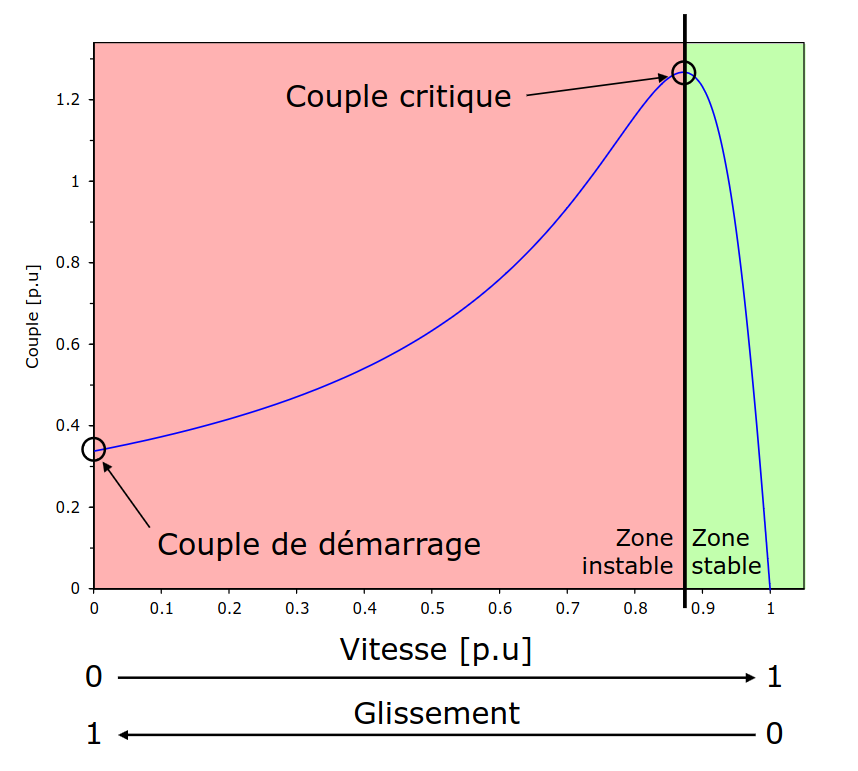
\includegraphics[width=.5\textwidth]{IMAGES/machineelec/couple.png}
\end{figure}

La zone instable est uniquement transitoire. La machine tourne uniquement si le couple à transmettre est inférieur au couple de démarrage.\\

Pour $s\rightarrow 0$ soit $v\rightarrow 1$, on a : \begin{equation}
    T_{em} \simeq \frac{3 U_e^2}{\Omega_s} \frac{s}{R_r'}
\end{equation}

On peut également trouver un couple et un glissement critique. (maximum de la courbe) : \begin{equation}
    \begin{gathered}
        s_k = \frac{R_r'}{\sqrt{R_e^2 + (X_e + X_{\sigma r})^2}}\\
        T_k = \frac{3U_e^2}{2\Omega_s [R_e + \sqrt{R_e^2 + (X_e + X_{\sigma r}')^2}]}\\
    \end{gathered}
\end{equation}

\subsubsection{Impédance équivalente}
On néglige ici l'influence de $R_{fer}$ car en pratique (même pour les plus petites machines), on a $R_{fer} > 20 X_h$ au minimum. \\

\begin{equation}
    Z_{eq} = R_s + j X_{\sigma s} + \frac{jX_h(\frac{R_r'}{s} + j X_{\sigma r}')}{jX_h + (\frac{R_r'}{s} + jX_{\sigma r}')}
\end{equation}

\begin{figure}[hbt!]
    \centering
    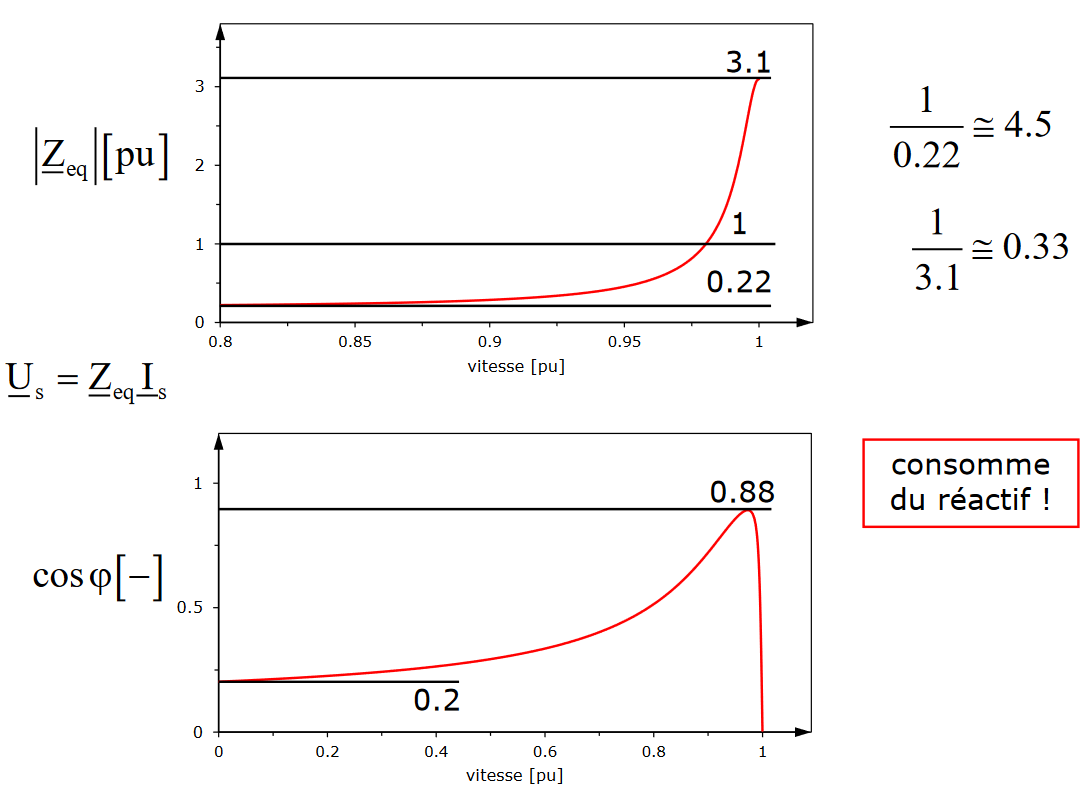
\includegraphics[width=.7\textwidth]{IMAGES/elec/elecimpe.png}
\end{figure}

\warning Au démarrage de la machine, on a donc un appel important de courant ! Celui-ci se stabilise ensuite à environ $1/3$ de la valeur nominale. Il faut donc faire attention lors du démarrage d'avoir l'ampérage nécessaire.\\

\subsubsection{Démarrage d'un moteur à cage}
Il existe différentes techniques pour réduire le courant au démarrage : \begin{itemize}
    \item Démarrage étoile/triangle : un moteur fonctionnant en triangle est câblé en étoile lors du démarrage\\
    \item Démarrage par auto-transformateur : insertion d'un abaisseur de tension\\
    \item Démarrage par impédance additionnelle : une résistance/inductance est ajoutée en série avec le stator\\
    \item Soft starter : convertisseur de puissance\\
\end{itemize}

\subsubsection{Mode de fonctionnement}
On peut changer la valeur du couple en \textbf{variant $U_s$ en amplitude}.\\

On peut changer la valeur de la vitesse du rotor (tout en gardant un couple constant) en \textbf{changeant $U_h$ et $f$ de telle sorte que $\frac{U_h}{f}$ reste constant.}\\
\warning Il s'agit bien ici de $U_h$ et non de $U_s$. En gardant le rapport $\frac{U_s}{f}$ constant, alors la courbe couple vs. vitesse ne se déplace plus uniquement selon l'axe des abscisses.\\

La machine peut également devenir génératrice lorsque $v$ [p.u] $>1$. On a alors la courbe inversée.\\

\begin{figure}[hbt!]
    \centering
    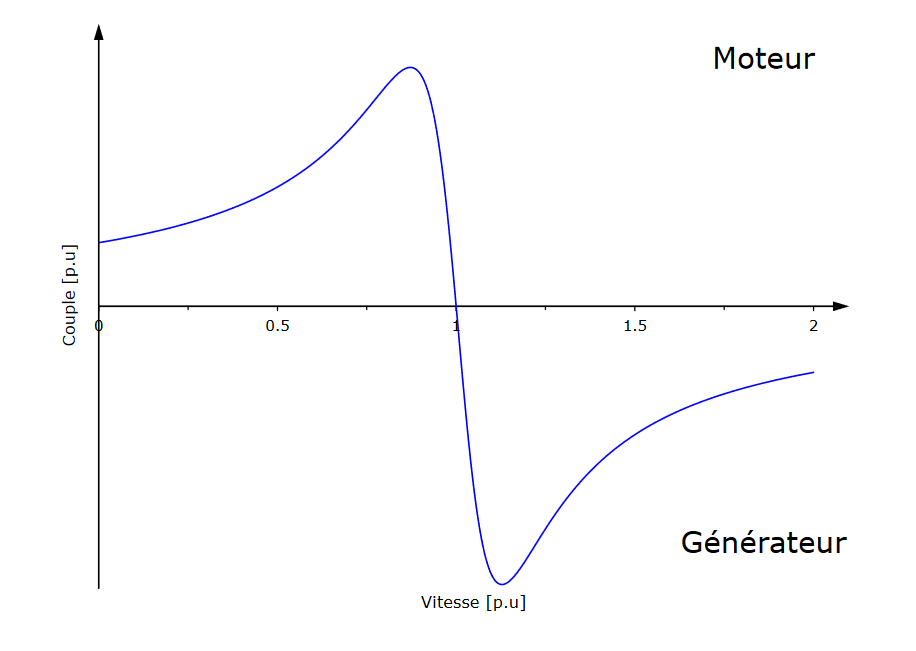
\includegraphics[width=.8\textwidth]{IMAGES/elec/generateurelec.png}
\end{figure}

Le bilan de puissance s'exprime alors de la même manière. Cependant, $P_{utile}$ et $P_{el}$ sont négatifs.\\


\subsection{Machine à courant continu}
La machine se compose de deux éléments : le stator (excitation) et le rotor (induit) qui possède un collecteur.\\
Une source DC fournit du courant au rotor via des charbons au collecteur. On utilise des charbons car c'est un bon conducteur qui résiste bien aux frottements. Cependant, il s'use essentiellement par la présence d'arcs électriques.\\

Le stator peut être formé d'aimants permanents tout comme de bobines.\\

\begin{figure}[hbt!]
    \centering
    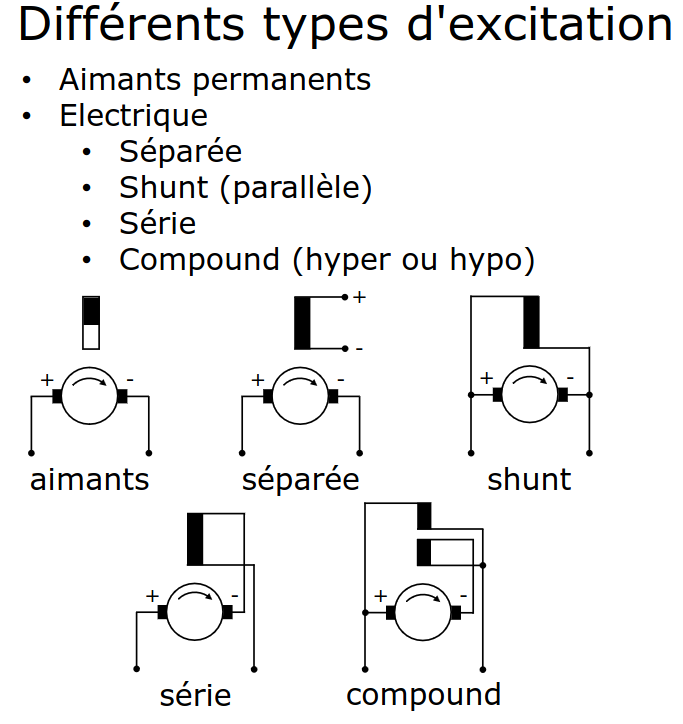
\includegraphics[width=.5\textwidth]{IMAGES/elec/mcc.png}
\end{figure}

Si l'on considère le régime permanent, on a pour l'excitation : $U_f = R_f I_f$\\

En régime permanent, le schéma équivalent est : \begin{figure}[hbt!]
    \centering
    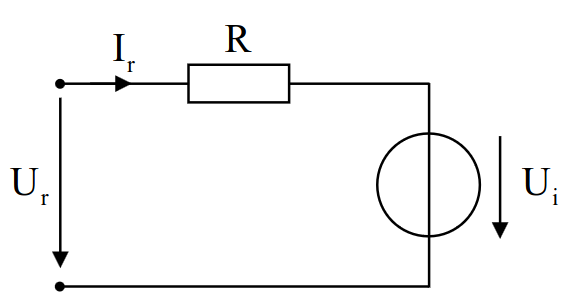
\includegraphics[width=.5\textwidth]{IMAGES/elec/mccschema.png}
\end{figure}

\begin{equation}
    U_r = R_r I_r + U_i
\end{equation}
Où $U_i$ est la tension induite de mouvement.\\

\begin{equation}
\begin{gathered}
    U_i = N \Omega p \hat{\Phi} = k_\phi \Omega\\
    k_\phi = k_{if} I_f\\
\end{gathered}
\end{equation}

La tension induite est donc proportionnelle à la vitesse de rotation et au courant d'excitation. De plus, si aimant permanent alors $k_\phi$ est constant.\\

Soit : $U_r = R_r I_r + k_\phi \Omega = R_r I_r + k_{if} I_f \Omega$\\

\subsubsection{Bilan de puissance}
\begin{equation}
    P_{el} = P_j + P_{em}
\end{equation}

\begin{itemize}
    \item $P_{el} = U_rI_r$\\
    \item $P_j = R_rI_r^2$\\
    \item $P_{em} = U_iI_r$\\
\end{itemize}

\begin{equation}
    T_{em} = \frac{U_iI_r}{\Omega} = k_\phi I_r = k_{if}I_f \Omega
\end{equation}

\begin{minipage}{.5\textwidth}
    \underline{Moteur :}\\
    $P_{el} >0$, $I_r >0$\\
    $T_{em} > 0$, $U_r > U_i$\\
\end{minipage}
\vline
\begin{minipage}{.5\textwidth}
    \underline{Génératrice :}\\
    $P_{el} < 0$, $I_r < 0$\\
    $T_{em} < 0$, $U_r < U_i$\\
\end{minipage}

\subsubsection{Excitation séparée}
On a ici $T_{em} = k_\phi \frac{U-k_\phi \Omega}{R}$\\

\begin{figure}[hbt!]
    \centering
    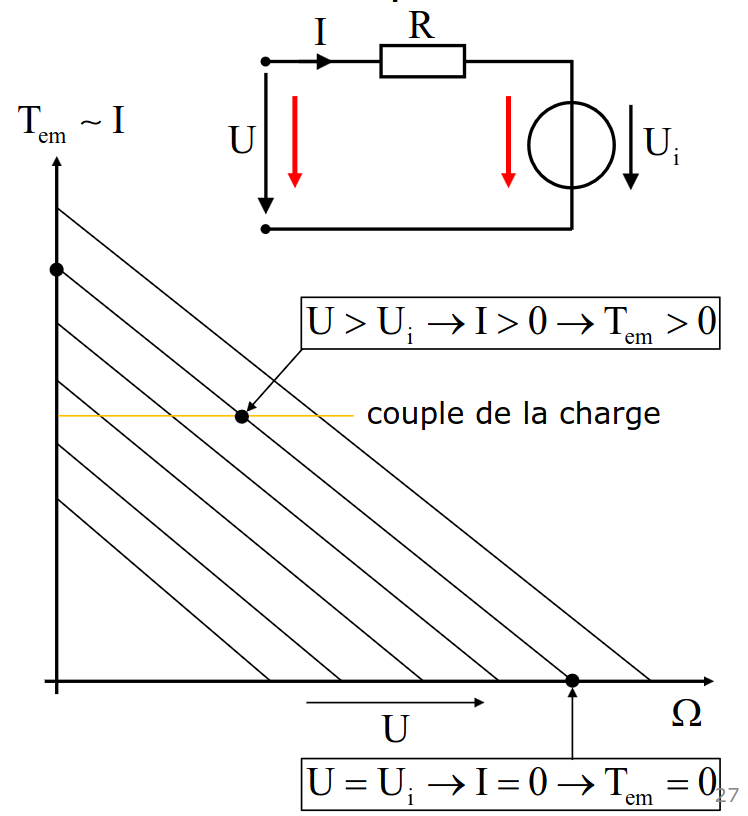
\includegraphics[width=.5\textwidth]{IMAGES/elec/excitationsep.png}
\end{figure}

Le couple est maximum pour une vitesse nulle et inversement. \\

\subsubsection{Aimants permanents}
$T_{em} = k_\phi I_r$\\
La caractéristique de couple est la même que pour l'excitation séparée.\\

\subsubsection{Excitation shunt (parallèle)}
$T_{em} = k_{if} I_f I_r$, $U_M = U_r = U_f$\\

\begin{figure}[hbt!]
    \centering
    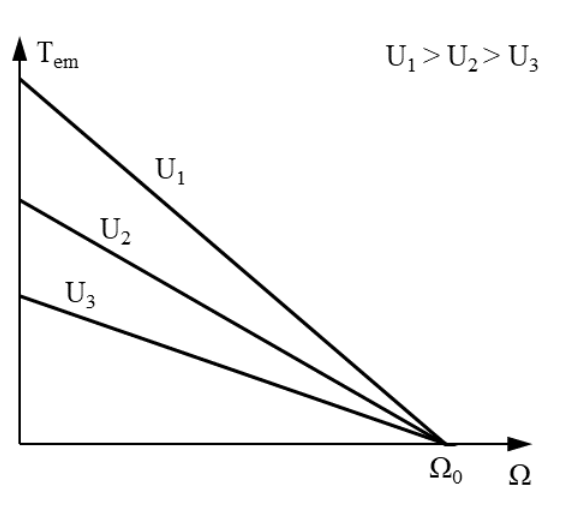
\includegraphics[width=.5\textwidth]{IMAGES/elec/mshunt.png}
\end{figure}

\subsubsection{Excitation série}
$T_{em} = k_{if} I_M^2$, $I_M = I_r = I_f$ \\

\begin{figure}[hbt!]
    \centering
    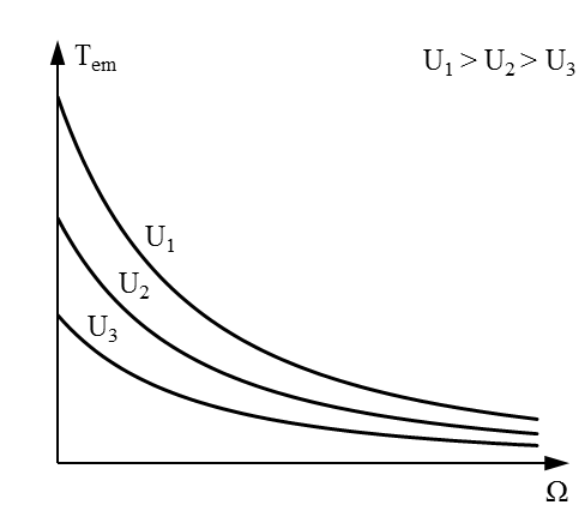
\includegraphics[width=.5\textwidth]{IMAGES/elec/mserie.png}
\end{figure}

\subsubsection{Excitation compound}
$T_{em} = k_{if} I_f I_r + k_{is} I_M^2$, $I_M = I_r+I_f$, $U_M = U_s+U_s$\\

\begin{figure}[hbt!]
    \centering
    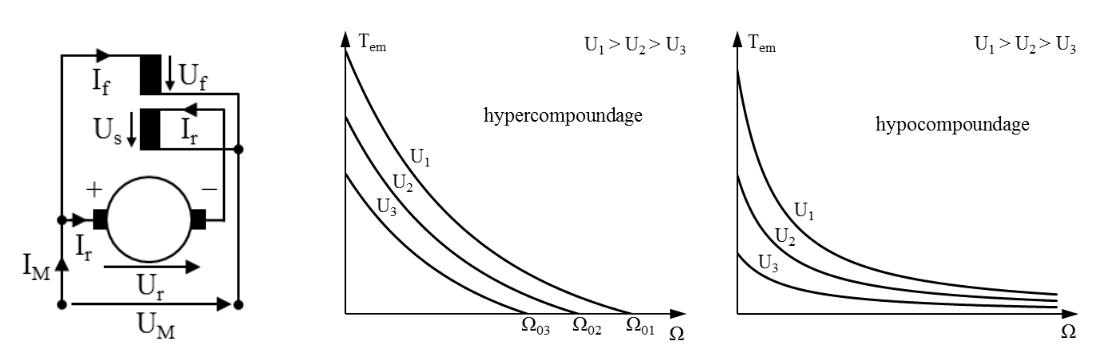
\includegraphics[width=.8\textwidth]{IMAGES/elec/mcompound.png}
\end{figure}

\subsubsection{Démarrage}
Lors du démarrage, le moteur à courant continu demande un courant selon une montée exponentielle!\\

\subsubsection{Moteur universel}
Le moteur à excitation série peut être alimenté en régime sinusoïdale. La caractéristique de couple devient alors plus faible que pour un régime continu.\\

\subsection{Machine synchrone}

Ici, le rotor est alimenté en DC. Il possède dès lors des bobines voire des aimants permanents. Le courant dans le rotor n'est donc pas induit.\\
L'excitation correspond donc ici au rotor.\\

\begin{equation}
    \Omega_s = \frac{\omega_s}{p}
\end{equation}
Avec $\Omega$, la vitesse dans le monde mécanique et $\omega$ dans le monde électrique. $n = \frac{f}{p}$\\

Deux types de machines synchrones : \begin{itemize}
    \item pôles lisses : le moyeu est plein\\
    \item pôles saillants : les bobines sont séparées par de l'air et le rotor n'a pas de forme cylindrique\\
\end{itemize}

On utilise principalement cette machine en \textbf{mode génératrice}. En effet, pour la démarrer, il faut de l'électronique.\\

\begin{itemize}
    \item Mode génératrice : $\delta>0$, où $\delta$ est l'angle entre les pôles du rotor et du stator\\
    \item Mode moteur : $\delta<0$\\
\end{itemize}

\subsubsection{Tension induite de mouvement}
\begin{equation}
    U_i = \sqrt{2} \pi N f \hat{\Phi} = k_\Phi \Omega = k_{if}I_f \Omega
\end{equation}

La tension induite de mouvement est proportionnelle à la vitesse de rotation et au courant d'excitation.\\

\subsubsection{Pôles lisses}
\begin{equation}
    \underline{U} = R\underline{I} + j X_d \underline{I}+ \underline{U}_i
\end{equation}
Avec $X_d = X_\sigma + X_h$\\
On néglige en général R car $R<<X_d$.\\

\begin{equation}
    P_{el} = P_j + P_{em}
\end{equation}
Avec \begin{itemize}
    \item $P_j = 3RI^2$\\
    \item $P_{em} = T_{em}\Omega_s$\\
    \item $P_{el} = 3UI\cos(\phi)$\\
\end{itemize}

\begin{equation}
    T_{em} = (3UI\cos(\phi)-3RI^2) \frac{1}{2\pi n_s} \rightarrow T_{em} = \frac{3UI\cos(\phi)}{2\pi n_s}
\end{equation}

Or, comme U est réel, on peut trouver que $I\cos\phi = \frac{U_i}{X_d}\sin \delta$\\

\begin{equation}
\begin{gathered}
    T_{em} = 3 \frac{U U_i}{2\pi n_s X_d}\sin \delta\\
    T_k = 3 \frac{UU_i}{2\pi n_s X_d}
    \end{gathered}
\end{equation}
Avec $T_k$, le couple maximal.\\

\begin{figure}[hbt!]
    \centering
    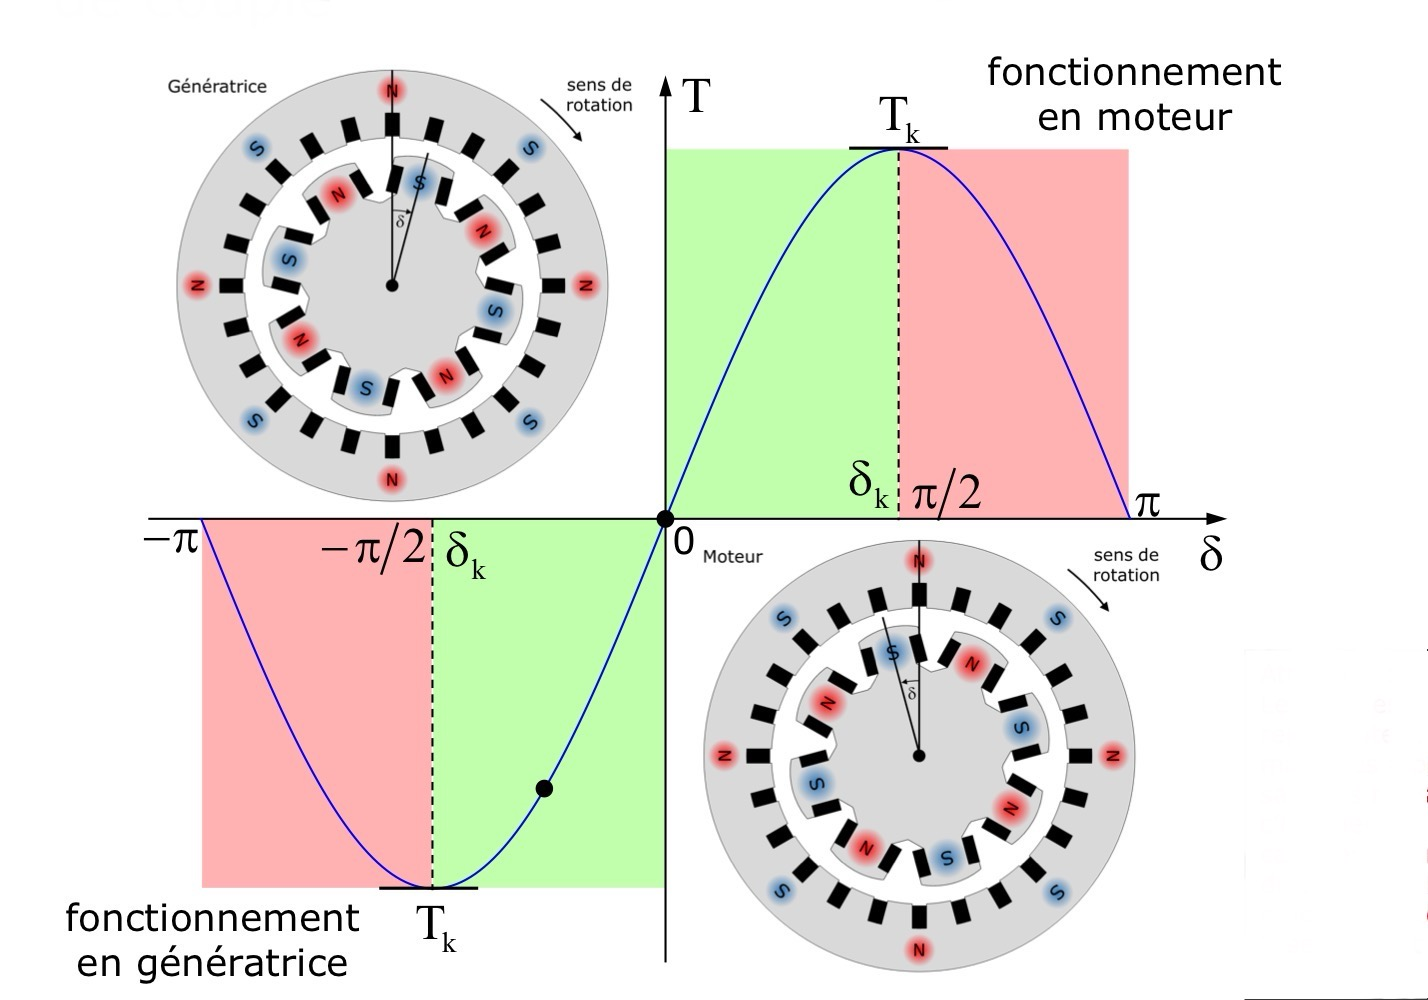
\includegraphics[width=.6\textwidth]{IMAGES/machineelec/IMG_0146.jpeg}
\end{figure}

\subsubsection{Pôles saillants}
L'analyse de cette machine demande des connaissances supplémentaires en analyse. On se contente d'énoncer les résultats.\\

Comme l'entrefer n'est pas constant, on a deux axes, d (peu d'entrefer) et q (beaucoup d'entrefer).\\
\begin{equation}
    \underline{U} = R\underline{I} + jX_dI_d - X_q I_q + \underline{U}_i
\end{equation}


La caractéristique de couple est alors : \\
\begin{equation}
    T_{em} = \frac{3}{2\pi n_s} [\frac{UU_i\sin \delta}{X_d} + \frac{U^2}{2} (\frac{1}{X_q}-\frac{1}{X_d})\sin(2\delta)]
\end{equation}

\begin{figure}[hbt!]
    \centering
    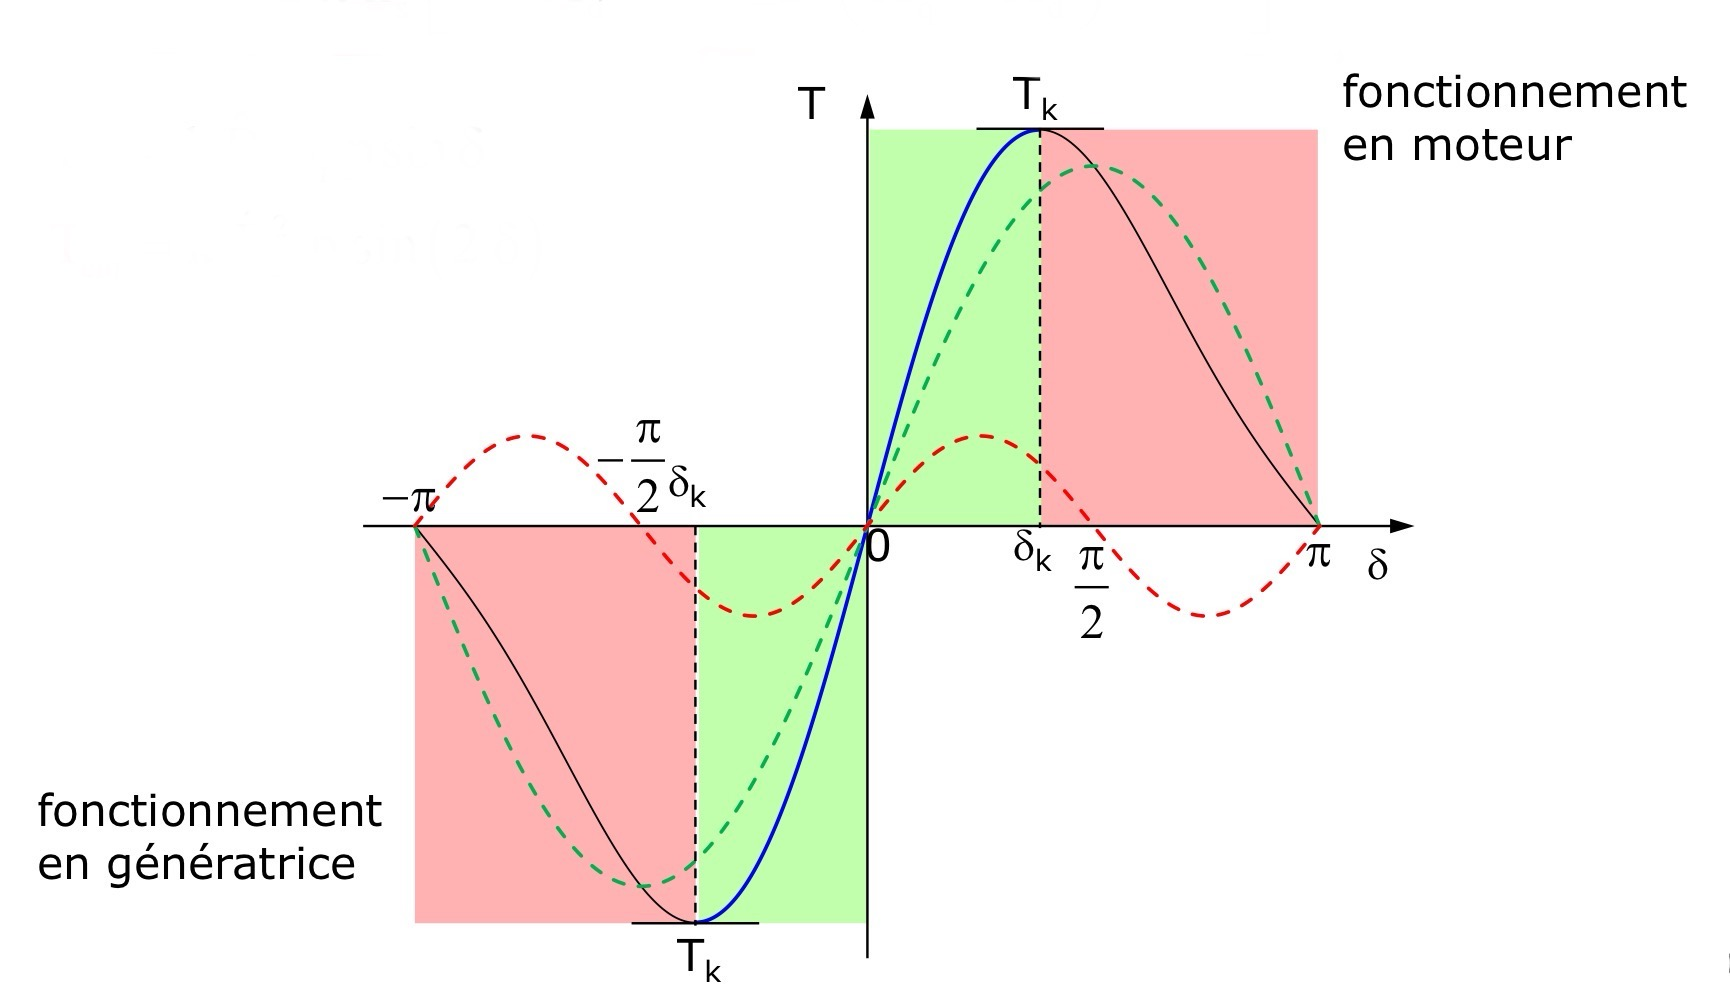
\includegraphics[width=.6\textwidth]{IMAGES/machineelec/IMG_0147.jpeg}
\end{figure}

Le couple est plus important avant le décrochage.\\
\subsubsection{Synchronisation au réseau}
Il y a plusieurs conditions pour une synchronisation au réseau : \begin{itemize}
    \item vitesse égales\\
    \item amplitude égales\\
    \item phase égales\\
    \item sens égaux\\
\end{itemize}

Pour que la machine synchrone puisse délivrer sur le réseau, ces trois conditions doivent être remplies, sinon il y aura de la casse matériel. \\

On peut définir : $I_{f0}$ le courant d'excitation à vide. C'est le courant d'excitation qu'il faut mettre pour avoir à vide la tension nominale du réseau.\\

\subsubsection{Topo-gramme (diagramme des puissances)}

\begin{figure}[hbt!]
    \centering
    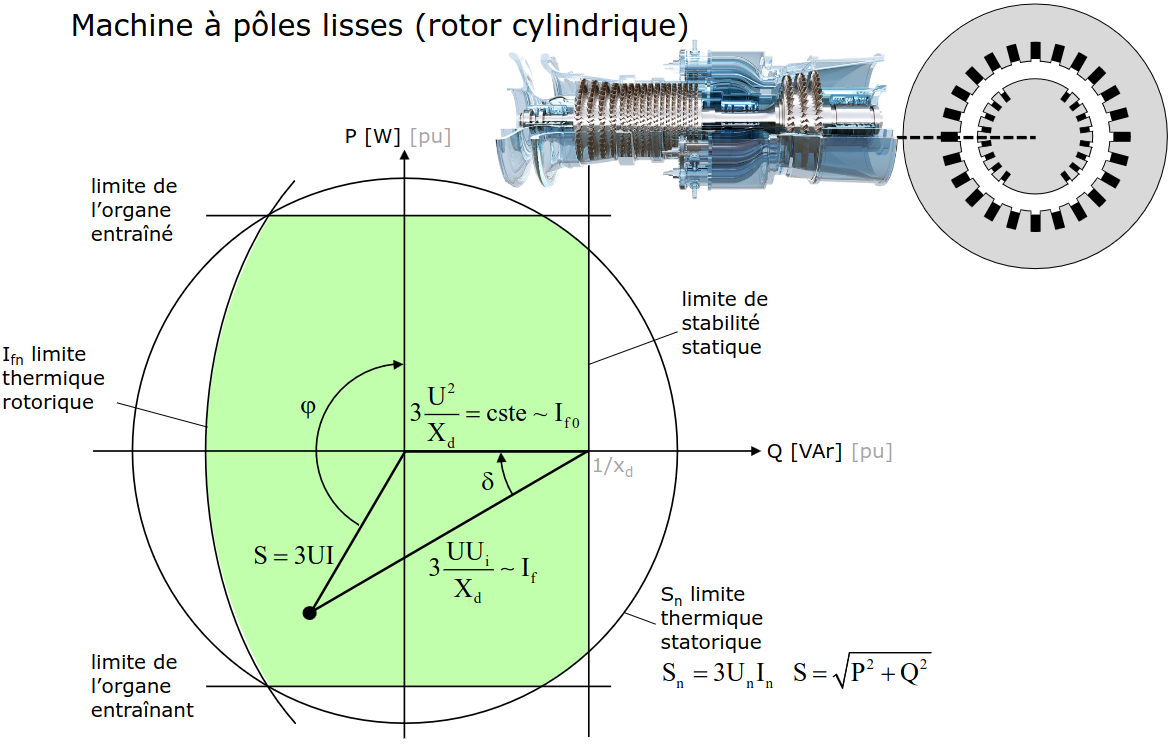
\includegraphics[width=.7\textwidth]{IMAGES/machineelec/Screenshot from 2023-11-16 23-32-03.png}
\end{figure}

Pour savoir où l'on se trouve sur dans le graphe, on forme des cercles à partir du point $\frac{1}{x_d}$. Plus on augmente l'excitation, plus le rayon du cercle devient important et plus on change le couple, plus on se déplace le long de ce cercle.\\

Les différentes limites sont des limites mécaniques et électriques.\\


\begin{figure}[hbt!]
    \centering
    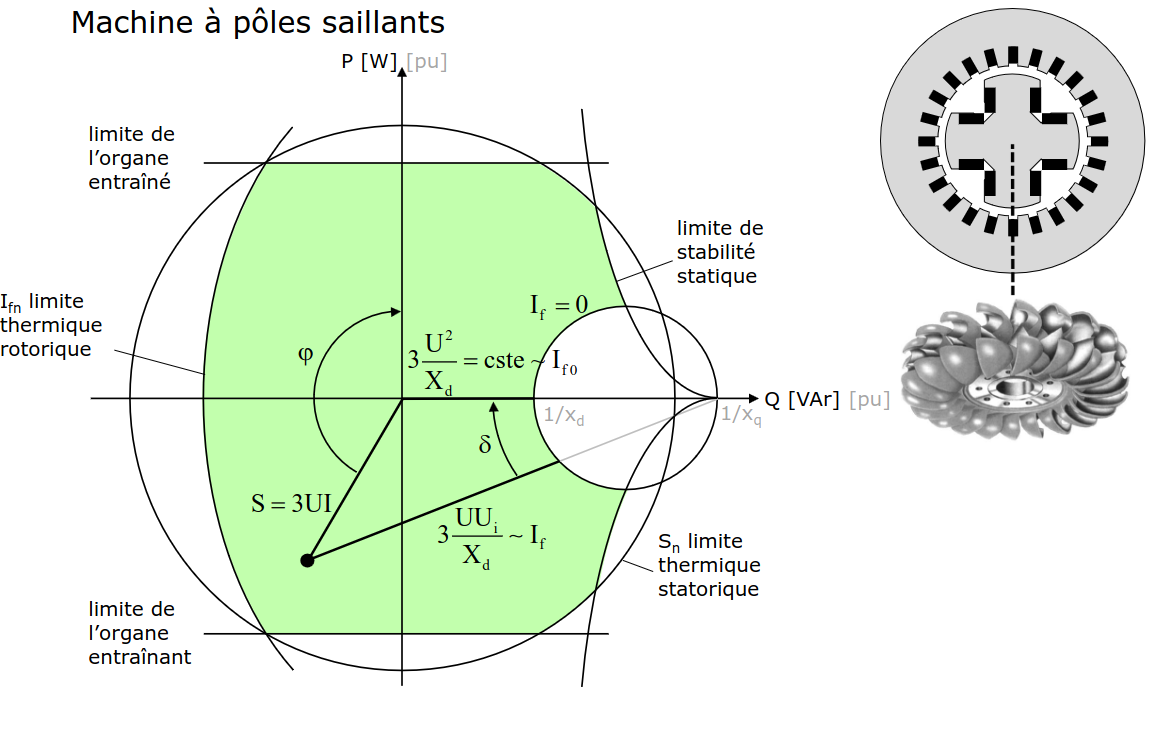
\includegraphics[width=.7\textwidth]{IMAGES/machineelec/Screenshot from 2023-11-16 23-35-24.png}
\end{figure}

Le graphe est ici similaire, cependant on trouve un cercle en $\frac{1}{x_d}$ et $\frac{1}{x_q}$.\\
Il s'agit ici d'un cas particulier du graphe précèdent où le point s'est transformé en cercle.\\

\subsection{Moteur synchrone à aimants permanents}

On utilise ici de l'électronique de puissance afin de moduler la fréquence pour que la position du stator vis à vis de celle du rotor soit toujours optimal.\\

Dans le cas présent, on a la tension induite : $U_i = k_\phi \Omega$ avec $k_\phi$ constant.\\

Soit : $u = Ri + L \frac{di}{dt} + u_i$\\
\warning Attention, ici l'inductance est variable comme la fréquence varie : $X_s = \omega_s L_s$\\

Comme la machine est alimentée en triphasée, on a comme puissance : \\
\begin{equation}
    \begin{gathered}
        P_{el} = P_j + P_{em} = 3UI\cos\phi\\
        P_j = 3RI^2\\
        P_{em} = 3U_iI\cos\psi\\
        T_{em} = 3k_\phi I \cos\psi\\
    \end{gathered}
\end{equation}

\warning Dans la pratique, on désire à $99\%$ du temps que $\cos \psi = 0$ (MTPA : maximum torque per ampere) afin d'obtenir le meilleur rendement possible.\\

Lorsque $\psi = 0$, alors $U_i$ et $I$ sont en phase et les 2 champs sont à $90^\circ$; le couple est maximal.\\

En cas d'utilisation en tant que frein, on change juste l'avance de $90^\circ$ par un retard de $90^\circ$.\\

\subsubsection{Types de commutation et appellations}
Il existe deux types principaux de commutations et d'appellations : \begin{itemize}
    \item Commutation par blocs à $120^\circ$ : on émet trois signaux rectangulaire à forme sinusoïdale. On peut dès lors négliger l'inductance et on a : $T_{em} = k_{T_{em}} I \cos\psi$, \textbf{Brushless}\\
    \item Alimentation sinusoïdale : $T_{em} = 3k_\phi I \cos\psi$, de plus en plus utilisé mais aussi compliqué à coder et analyser pour aligner comme on le souhaite le stator et le rotor, \textbf{PMSM : Permanent Magnet Synchronous Machine}\\
\end{itemize}

\subsubsection{Caractéristique de couple}

\quad \underline{Commutation par blocs à $120^\circ$ :}\\

\begin{figure}[hbt!]
    \centering
    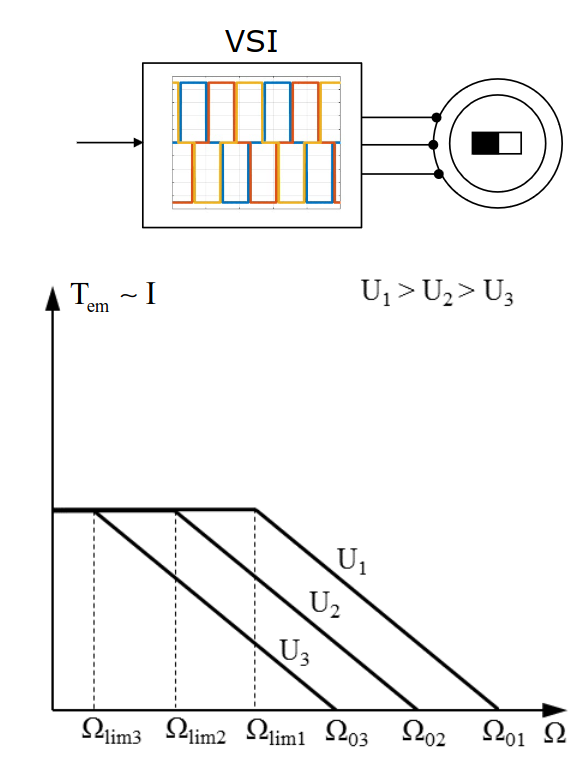
\includegraphics[width=.4\textwidth]{IMAGES/machineelec/Screenshot from 2023-11-25 00-38-51.png}
\end{figure}

On a un plateau avant la corner speed.\\

De la même manière, pour une alimentation sinus, on a la caractéristique suivante : \\

\begin{figure}[hbt!]
    \centering
    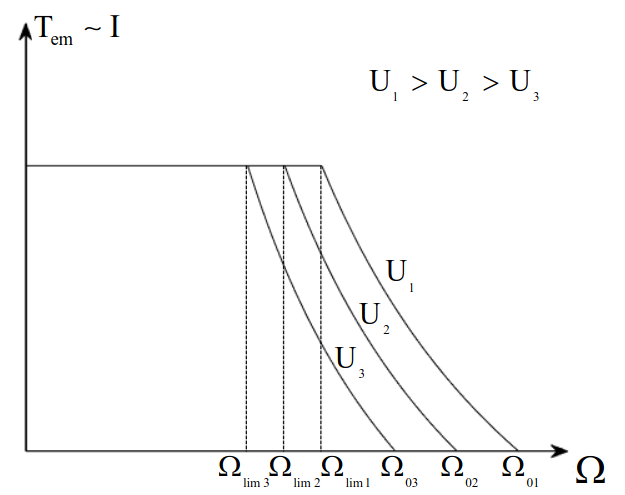
\includegraphics[width=.6\textwidth]{IMAGES/machineelec/Screenshot from 2023-11-25 00-42-03.png}
\end{figure}

\footnote{On peut également faire du défluxage; on réduit l'angle de $90^\circ$, ce qui diminue le couple à un instant donné mais permet de conserver un couple positif plus longtemps à grande vitesse.}

\subsection{Moteur pas à pas}
Il s'agit d'un moteur dont le rotor tourne par incréments discrets.\\
Trois types majeurs : \begin{itemize}
    \item Réluctant (équivalent machine synchrone à pôles saillants)\\
    \item Électromagnétique : \begin{itemize}
        \item à griffes\\
        \item Lavet (montre)\\
    \end{itemize}
    \item Hybride\\
\end{itemize}

\subsubsection{Moteur réluctant}
Rotor non cylindrique. \\
\textbf{Nombre de phases} le plus fréquent : 3,4,8\\
\textbf{Nombre de pas par tour} : 12-72\\
\warning Le couple produit est faible.\\
L'ordre d'alimentation est inverse au sens de rotation du rotor.\\

\begin{figure}[hbt!]
    \centering
    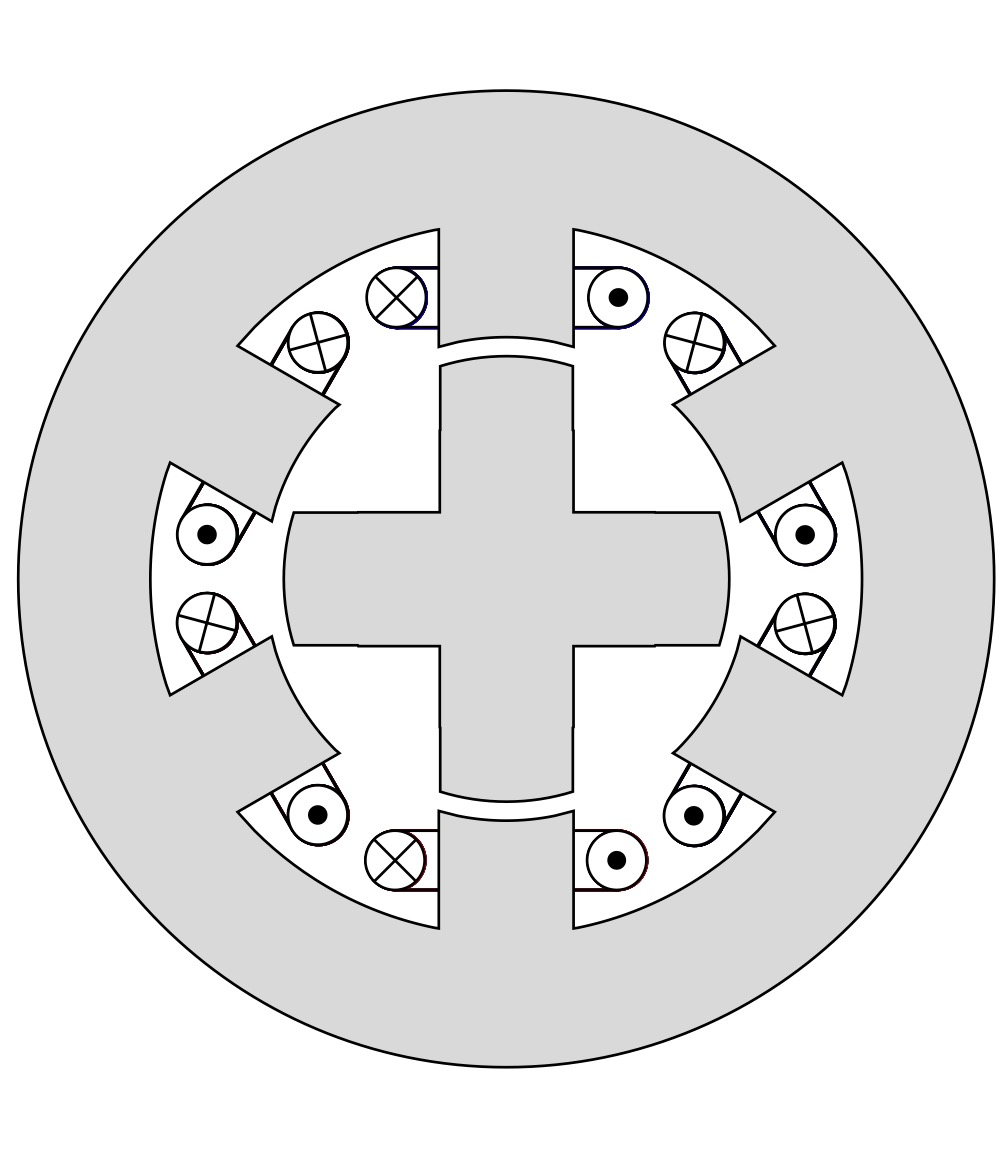
\includegraphics[width=.3\textwidth]{IMAGES/machineelec/IMG_0158.jpeg}
\end{figure}

\subsubsection{Moteur électromagnétique}
Habituellement biphasé. Rendement élevé.\\
\textbf{Nombre de pas par tour} : 2-24\\
Petit couple à l'arrêt.\\

Le rotor est un aimant permanent. \\

\quad \underline{Moteur à griffes :}\\

\begin{figure}[hbt!]
    \centering
    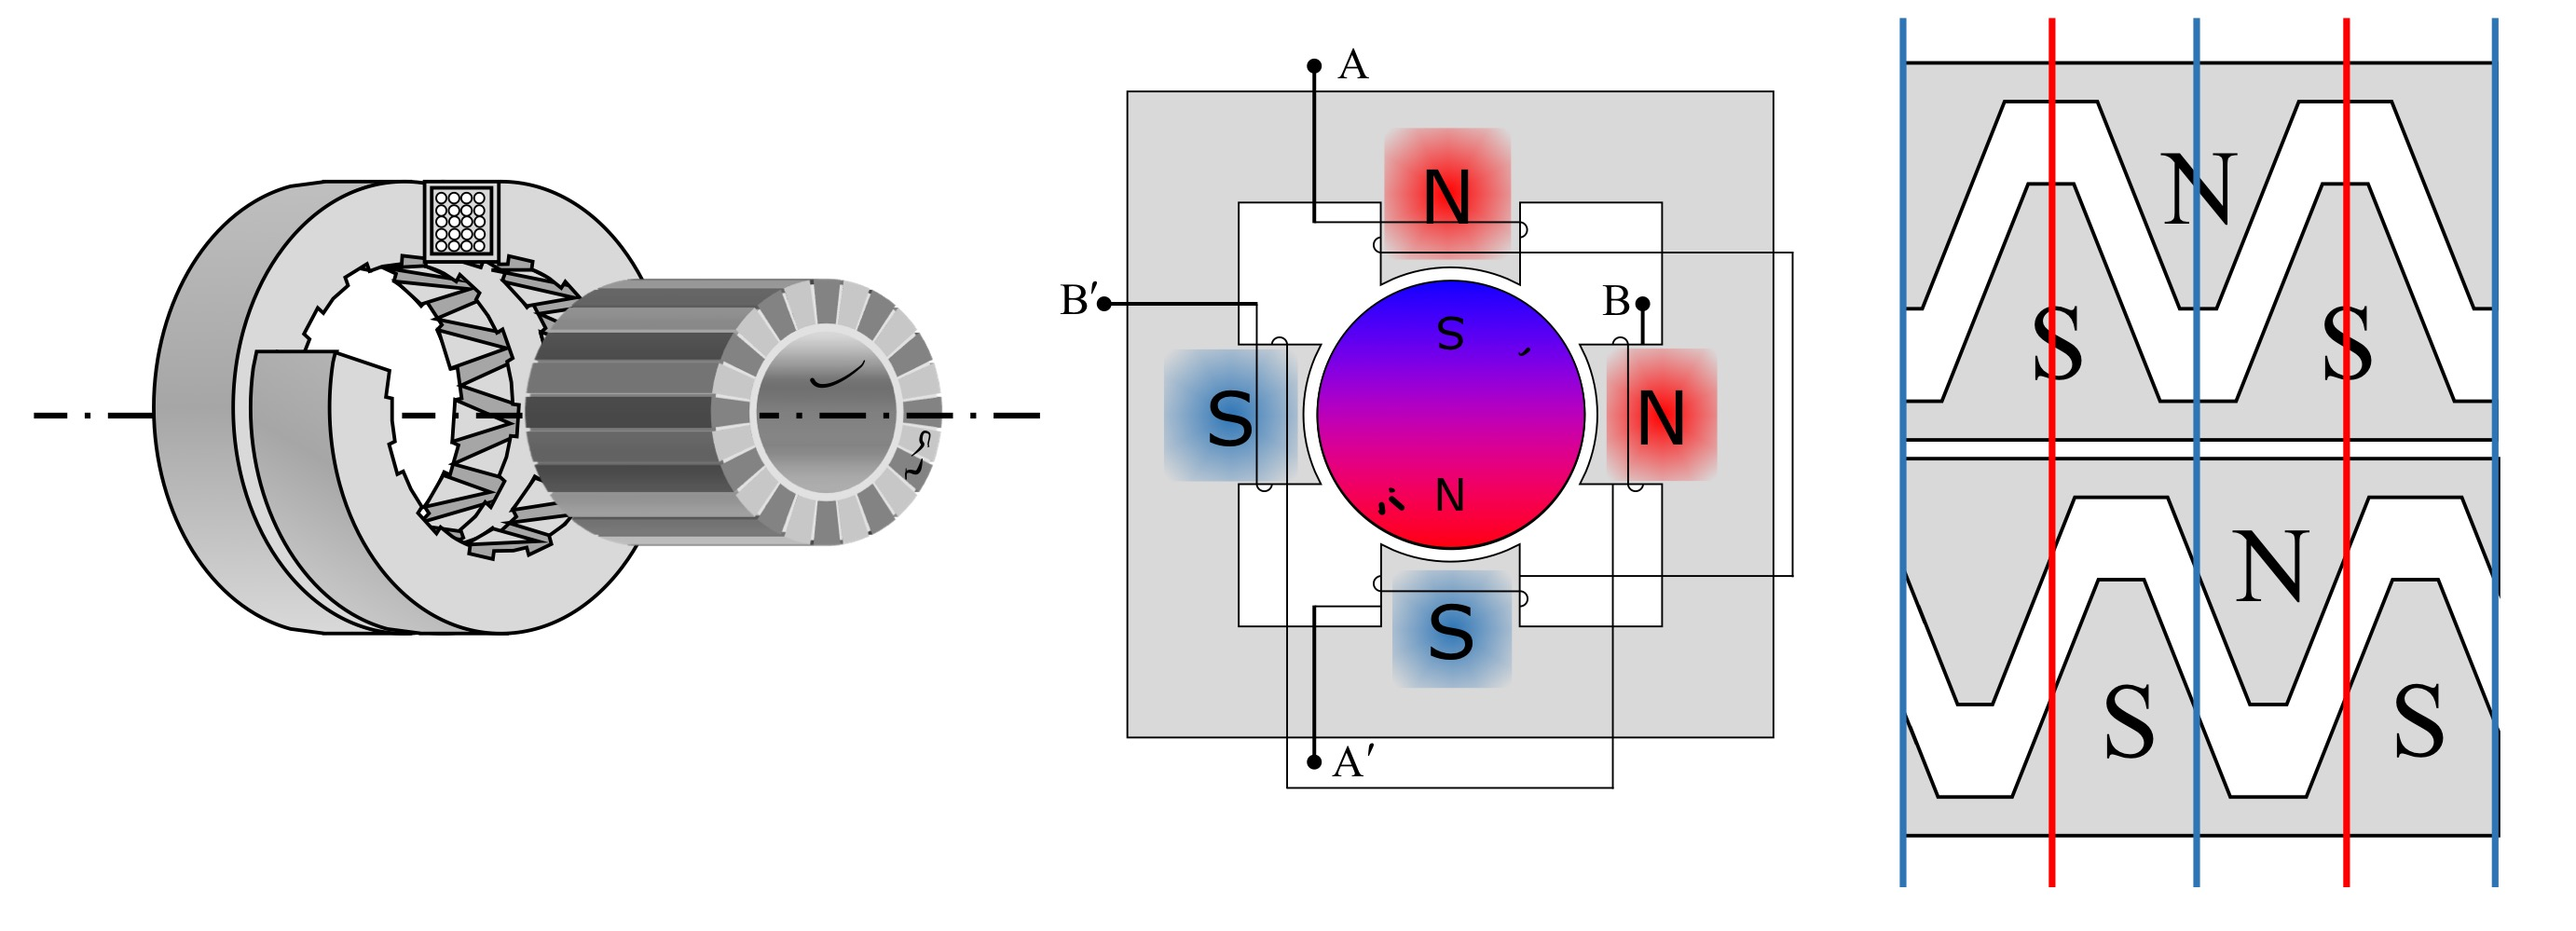
\includegraphics[width=.6\textwidth]{IMAGES/machineelec/IMG_0159.jpeg}
\end{figure}

Le nombre d'anneaux correspond au nombre de phases. Les triangles agissent comme des pôles lorsqu'un champ B les traverse.\\

\quad \underline{Moteur Lavet :}\\
Utilisé dans les montres. Il utilise la saturation du fer afin de faire tourner un aimant sur lequel est posé un rotor.\\
L'aimant au repos se trouve perpendiculaire aux encoches de positionnement. Lorsqu'un champ B est imposé, l'aimant s'aligne avec le champ et se met dans un équilibre instable de telle sorte que lorsque le champ est enlevé, l'aimant revient à une position d'équilibre stable.\\

\begin{figure}[hbt!]
    \centering
    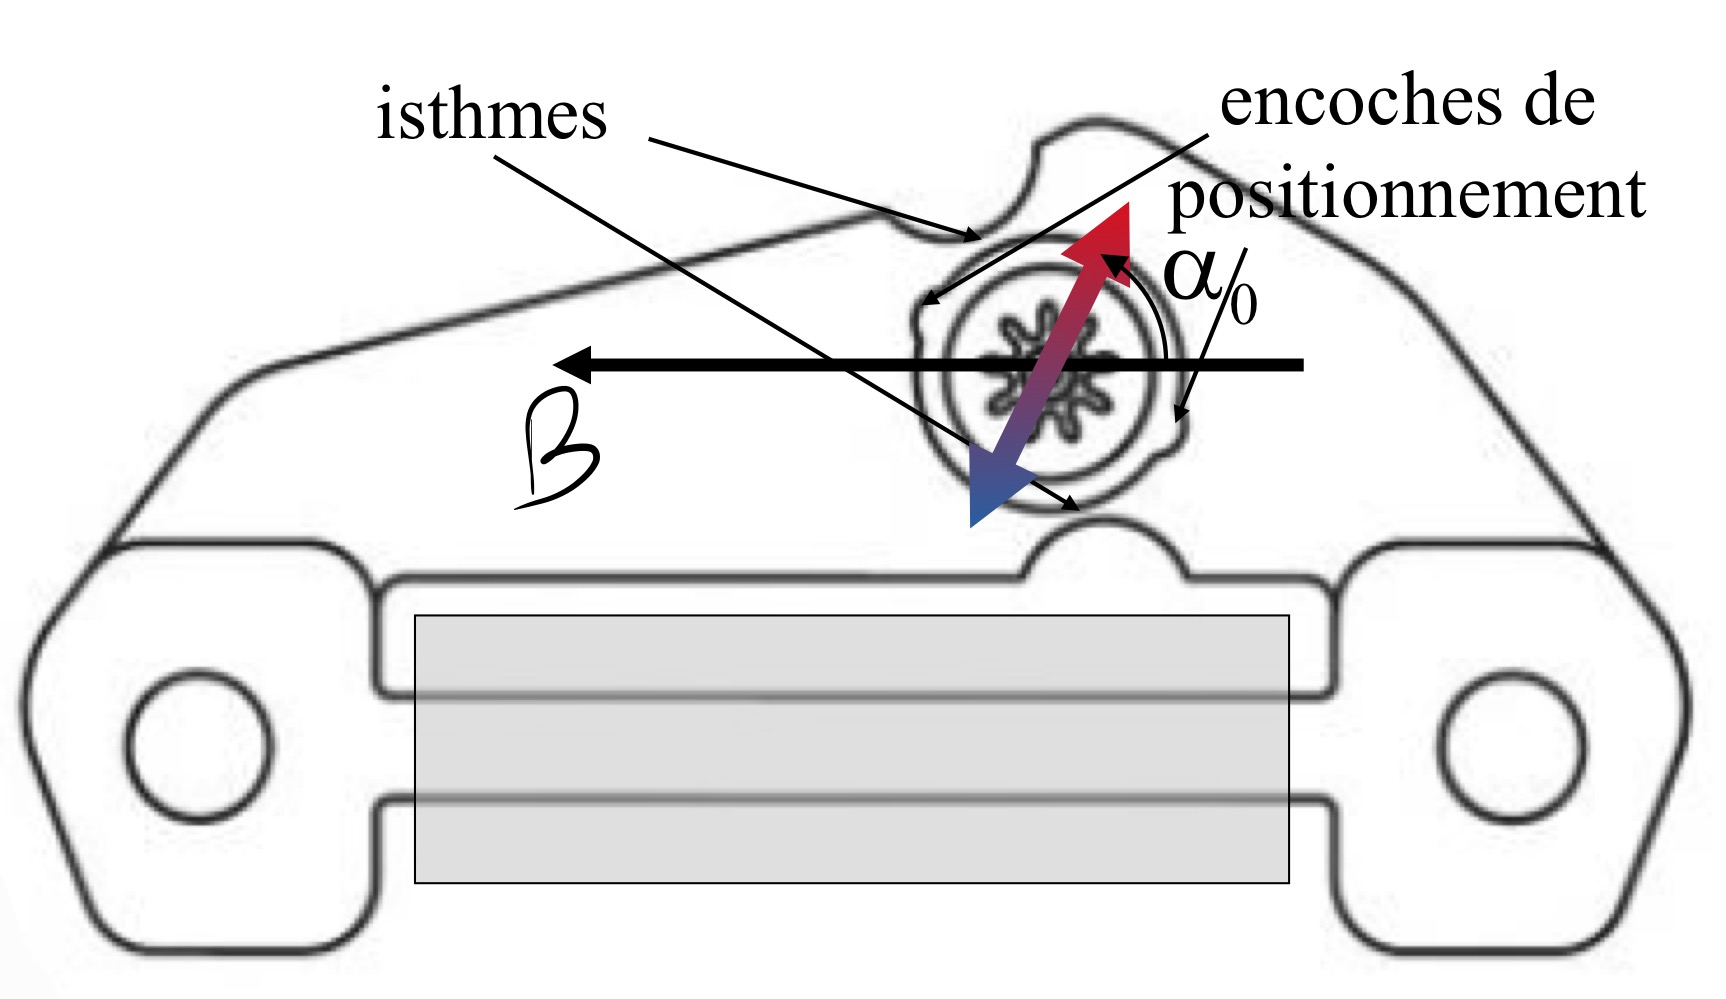
\includegraphics[width=.5\textwidth]{IMAGES/machineelec/IMG_0160.jpeg}
\end{figure}

\subsubsection{Moteur hybride (réluctant polarisé)}
\textbf{Nombre de pas par tour} : 24-400\\
Rendement bon\\

Un met deux engrenages décalés d'une dent sur le rotor. Chacun des engrenages est polarisé. Le décalage permet d'obtenir un couple important pour une taille réduite.\\

\begin{figure}[hbt!]
    \centering
    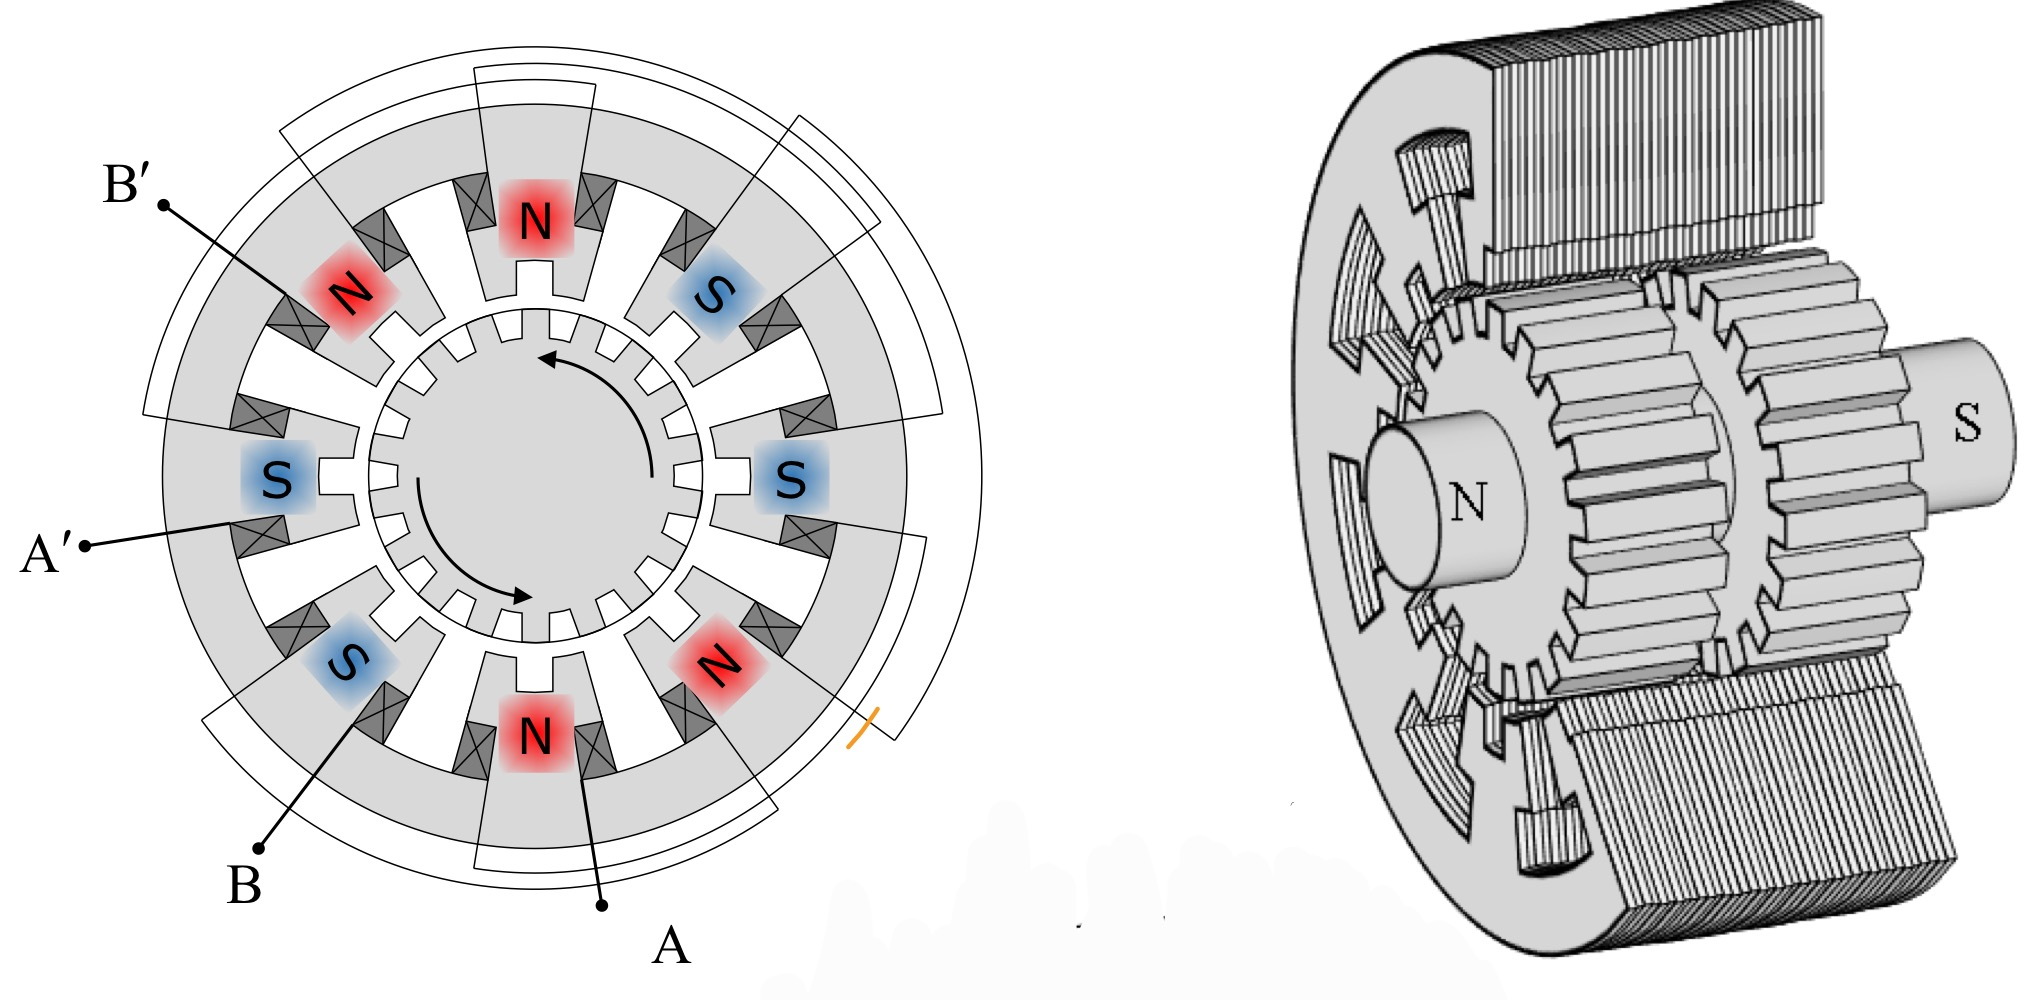
\includegraphics[width=.6\textwidth]{IMAGES/machineelec/IMG_0161.jpeg}
\end{figure}

\begin{figure}[hbt!]
    \centering
    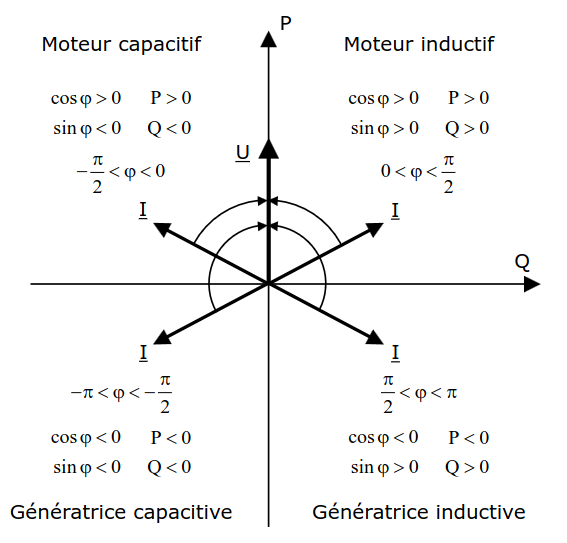
\includegraphics[width=.6\textwidth]{IMAGES/machineelec/Screenshot from 2024-01-13 12-35-56.png}

\end{figure}


\end{document}